% DiffuSAM — AIMed 2026 Poster
% A0 Portrait (841 mm × 1189 mm), readable from 2–3 m
% Visual style adapted from ISBI 2024 poster template.
% Structure mirrors the accepted abstract.
% Compile: pdflatex aimed2026_poster.tex
\documentclass[a0paper,portrait]{article}

\usepackage[a0paper,margin=1.6cm]{geometry}
\usepackage[T1]{fontenc}
\usepackage{lmodern}
\usepackage{graphicx}
\usepackage{booktabs}
\usepackage{tabularx}
\usepackage{array}
\usepackage{multicol}
\usepackage{enumitem}
\usepackage{caption}
\usepackage{xcolor}
\usepackage{tikz}
\usepackage{amsmath}
\usepackage{amssymb}
\usepackage{hyperref}
\hypersetup{colorlinks=false}

% ── Colour palette ─────────────────────────────────────────────
\definecolor{SectionBlue}{HTML}{156082}
\definecolor{DarkBlue}{HTML}{0E2841}
\definecolor{AccentOrange}{HTML}{E97132}
\definecolor{LightGray}{HTML}{F5F5F5}
\definecolor{PlaceGray}{HTML}{BBBBBB}

% ── Font sizes for A0 ─────────────────────────────────────────
\renewcommand{\normalsize}{\fontsize{28}{35}\selectfont}
\renewcommand{\small}{\fontsize{24}{30}\selectfont}
\renewcommand{\footnotesize}{\fontsize{20}{25}\selectfont}
\renewcommand{\large}{\fontsize{35}{43}\selectfont}
\renewcommand{\Large}{\fontsize{44}{52}\selectfont}
\renewcommand{\LARGE}{\fontsize{54}{62}\selectfont}
\renewcommand{\huge}{\fontsize{66}{74}\selectfont}
\renewcommand{\Huge}{\fontsize{78}{86}\selectfont}
\normalsize

\setlength{\parindent}{0pt}
\setlength{\parskip}{0.25em}
\setlength{\columnsep}{1.4cm}
\newcolumntype{Y}{>{\centering\arraybackslash}X}
\newcolumntype{Z}{>{\raggedright\arraybackslash}X}

% ── Section header (column-width blue bar) ─────────────────────
\newcommand{\sectionbar}[1]{%
  \vspace{0.20cm}%
  \begin{tikzpicture}
    \node[
      fill=SectionBlue,
      rounded corners=10pt,
      inner xsep=18pt,
      inner ysep=8pt,
      text=white,
      font=\large\bfseries,
      minimum width=\columnwidth,
      anchor=west
    ] at (0,0) {#1};
  \end{tikzpicture}%
  \vspace{0.20cm}\par%
}

% ── Full-width section header (footer) ─────────────────────────
\newcommand{\sectionbarwide}[1]{%
  \vspace{0.1cm}%
  \begin{tikzpicture}
    \node[
      fill=SectionBlue,
      rounded corners=10pt,
      inner xsep=18pt,
      inner ysep=8pt,
      text=white,
      font=\large\bfseries,
      minimum width=\textwidth,
      anchor=west
    ] at (0,0) {#1};
  \end{tikzpicture}%
  \vspace{0.06cm}\par%
}

\pagestyle{empty}

\begin{document}

% ================================================================
%  HEADER BANNER (drawn as TikZ overlay so logos stay inside)
% ================================================================
\begin{tikzpicture}[remember picture, overlay]
  \fill[DarkBlue]
    ([yshift=0pt]current page.north west) rectangle
    ([yshift=-385pt]current page.north east);
  \draw[AccentOrange, line width=5pt]
    ([yshift=-385pt]current page.north west) --
    ([yshift=-385pt]current page.north east);
\end{tikzpicture}

\vspace*{0.7cm}
\noindent
\begin{minipage}[c][8.9cm][c]{0.14\textwidth}
  \centering
  
\includegraphics[width=0.96\linewidth]{tau_logo.png}
\end{minipage}\hfill
\begin{minipage}[c][8.9cm][c]{0.70\textwidth}
  \begin{center}
  {\color{white}\LARGE\bfseries
  DiffuSAM: Diffusion-Based Prompt-Free SAM2 for\\[6pt]
  Few-Shot and Source-Free Medical Image Segmentation}

  \vspace{8pt}

  {\color{white}\Large
  Tal Grossman$^{1,\dagger}$ \quad
  Noa Cahan$^{1,\dagger}$ \quad
  Lev Ayzenberg$^{1}$ \quad
  Hayit Greenspan$^{2}$}

  \vspace{6pt}

  {\color{white}\small
  $^{\dagger}$Equal contribution \hspace{1.0em}
  $^{1}$School of Electrical Engineering, Tel Aviv University, Israel \hspace{1.0em}
  $^{2}$School of Biomedical Engineering, Tel Aviv University, Israel}

  \vspace{4pt}

  {\color{white}\small
  \texttt{talgrossman22@gmail.com, hayit@eng.tau.ac.il}}
  \end{center}
\end{minipage}\hfill
\begin{minipage}[c][8.9cm][c]{0.14\textwidth}
  \centering
  % Right-logo placeholder reserved intentionally (no drawing on poster):
  % \includegraphics[width=0.96\linewidth]{placeholder_logo.png}
\end{minipage}

% \vspace{1.35cm}
\vspace{2cm}

% ================================================================
%  TWO-COLUMN BODY
% ================================================================
\begin{multicols}{2}

% ── LEFT COLUMN ────────────────────────────────────────────────

\sectionbar{Key Information}

\textbf{\color{SectionBlue}Research question}\\
Can a lightweight diffusion prior over frozen SAM2 features enable accurate prompt-free medical image segmentation in both few-shot learning and source-free unsupervised domain adaptation, without full fine-tuning or expert-provided prompts?

\vspace{4pt}
\textbf{\color{SectionBlue}Findings}\\
DiffuSAM achieves \textbf{87.2\%} average Dice in few-shot CT segmentation and \textbf{85.2\%} in source-free CT-to-MRI domain adaptation on abdominal organs, competitive with state-of-the-art methods while requiring $<$5\,GB GPU memory and no user prompts.

\vspace{4pt}
\textbf{\color{SectionBlue}Meaning}\\
Diffusion-based memory generation offers a practical, lightweight path for adapting vision foundation models to medical imaging without prompts or expensive fine-tuning, facilitating clinical workflow integration.

\vspace{0.5cm}
\sectionbar{Introduction}

Medical image segmentation is vital for clinical diagnosis and treatment planning.
Foundation models such as SAM\,[1] and SAM2\,[2] achieve strong zero-shot performance on natural images but struggle with medical data due to domain differences in texture, contrast, and anatomy.
Their reliance on expert-provided prompts further limits clinical deployment.
Prior adaptations such as MedSAM\,[3] require costly fine-tuning and typically still depend on prompts. This challenge is especially acute in source-free unsupervised domain adaptation, where models must adapt across modalities without access to source-domain images.

\vspace{4pt}
\textbf{We propose DiffuSAM}, a diffusion-based framework for \textbf{prompt-free} medical image segmentation and \textbf{source-free domain adaptation} that keeps the SAM2 backbone \textbf{entirely frozen}.

\vspace{0.5cm}
\sectionbar{Material and Methods}

DiffuSAM trains a lightweight UNet-based diffusion prior conditioned on frozen SAM2 image encoder features and class labels to generate SAM2-compatible memory embeddings.
These embeddings are injected into SAM2's memory attention and mask decoder, producing segmentation masks without user prompts.

\vspace{4pt}
For volumetric consistency in 3D scans, the prior is additionally conditioned on predictions from adjacent slices, propagating bidirectionally from the center slice.
The SAM2 backbone remains entirely frozen; only the compact diffusion prior is trained, requiring \textbf{$<$5\,GB GPU memory} and converging in \textbf{under 8{,}000 iterations}.

\vspace{0.08cm}
\begin{center}
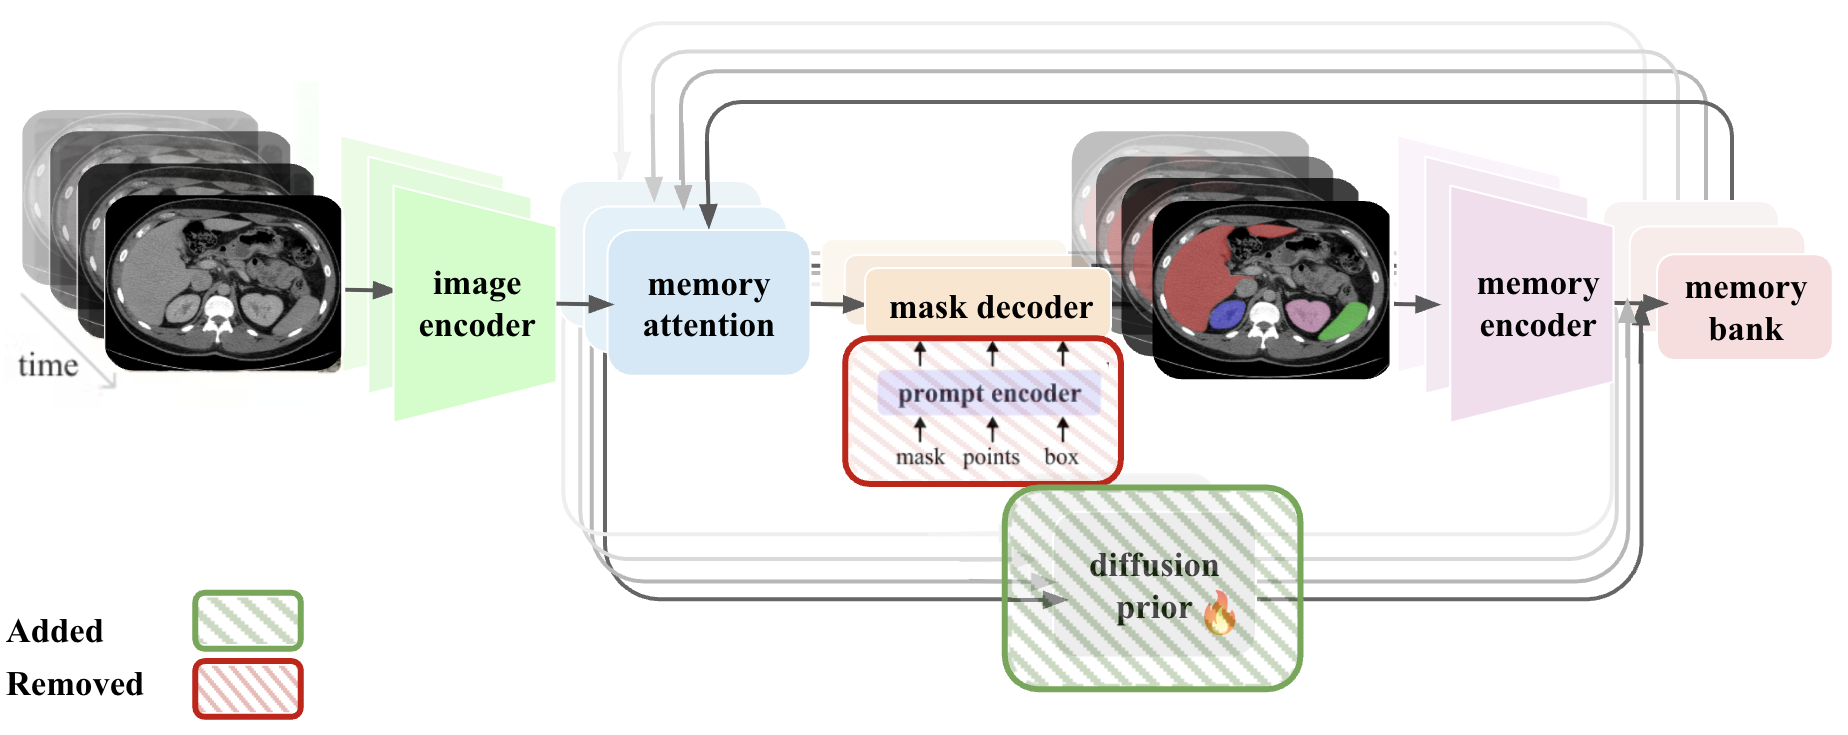
\includegraphics[width=0.90\columnwidth]{pipeline_a_cropped.png}
\end{center}
\vspace{1pt}
{\small\textit{DiffuSAM overview.} The diffusion prior generates SAM2-compatible memory embeddings from frozen image features, removing the prompt encoder from the adaptation path.}

\vspace{0.04cm}
\begin{center}
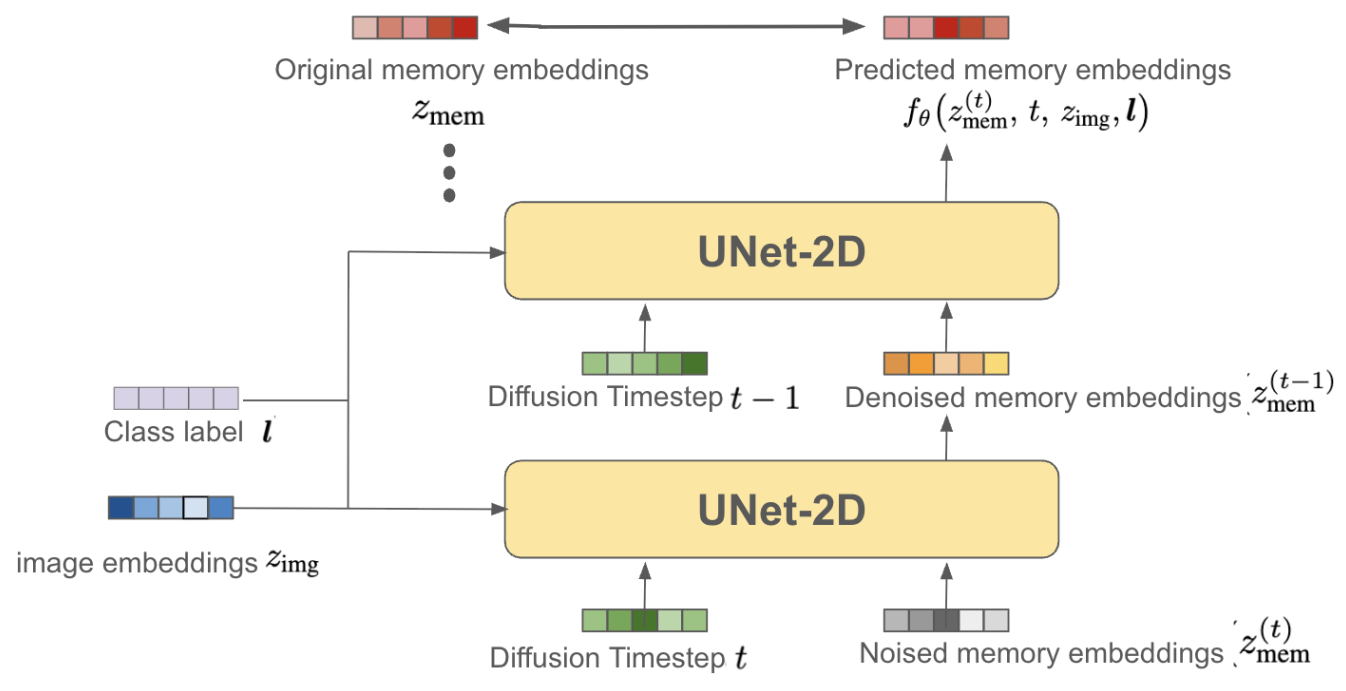
\includegraphics[width=0.72\columnwidth]{pipeline_b_cropped.png}
\end{center}
\vspace{1pt}
{\small\textit{Diffusion prior training and sampling.} A UNet denoises memory embeddings conditioned on timestep, image embedding, and class label, then samples a predicted memory in two steps.}

\vspace{1.5cm}
{\small
A simple \textbf{L2 loss} trains the \textbf{prior} to recover the clean memory embedding from a noised version conditioned on image features, timestep, and class label.
We also add a \textbf{segmentation loss} on decoded masks from synthesized memory embeddings passed through frozen SAM2 memory attention and the mask decoder.
\[
\mathcal{L}_{\text{prior}}
=
\begin{aligned}[t]
&\mathbb{E}_{t\sim[1,T],\, z_{\text{mem}}^{(t)}\sim q_t}
\left\| f_{\theta}\!\left(z_{\text{mem}}^{(t)},\, t,\, z_{\text{img}},\, \mathbf{l}\right)
- z_{\text{mem}} \right\|_2^2
\end{aligned}
\]
\vspace{-4cm}
\[
\mathcal{L} = \lambda_{\text{prior}} \mathcal{L}_{\text{prior}} +
\lambda_{\text{seg}} \mathcal{L}_{\text{seg}}
\]
}

% ── RIGHT COLUMN ───────────────────────────────────────────────
\columnbreak

\sectionbar{Results}

We evaluated DiffuSAM on the \textbf{BTCV}\,[9] (CT) and \textbf{CHAOS}\,[10] (MRI) abdominal datasets for spleen, kidney, and liver segmentation under:
\begin{itemize}[leftmargin=1em, itemsep=2pt, topsep=4pt]
\item \textbf{Few-shot:} 3 of 30 training volumes (BTCV)
\item \textbf{Source-free UDA:} CT\,$\to$\,MRI without target labels
\end{itemize}

\vspace{0.08cm}

{\small
\captionsetup{font=small, labelfont=bf}
\captionof{table}{Few-shot Dice scores (\%) on BTCV (3 training volumes).}
\vspace{2pt}
\centering
\renewcommand{\arraystretch}{1.15}
\begin{tabular*}{\columnwidth}{@{\extracolsep{\fill}}lccccc@{}}
\toprule
\textbf{Method} & \textbf{Spleen} & \textbf{R.Kidney} & \textbf{L.Kidney} & \textbf{Liver} & \textbf{Avg} \\
\midrule
UNet~[4]          & 54.85 & 55.99 & 48.70 & 85.85 & 61.35 \\
UNETR~[5]         &  8.65 &  0.24 &  2.14 & 78.15 & 22.30 \\
SAM~[1]           & 15.53 & 52.19 & 62.19 & 26.56 & 39.12 \\
SAM2~[2]          & 20.24 & 55.67 & 66.94 & 34.59 & 44.36 \\
FATE-SAM~[6]      & 86.22 & 90.99 & 89.32 & 82.17 & 87.18 \\
\midrule
DiffuSAM (w/o 3D) & 82.87 & 80.95 & 83.56 & 83.49 & 82.72 \\
\textbf{DiffuSAM} & \textbf{86.54} & 88.61 & 86.50 & \textbf{87.29} & \textbf{87.24} \\
\bottomrule
\end{tabular*}
}

\vspace{0.04cm}

{\small
\captionsetup{font=small, labelfont=bf}
\captionof{table}{Source-free UDA Dice scores (\%): BTCV CT\,$\to$\,CHAOS MRI.}
\vspace{2pt}
\centering
\renewcommand{\arraystretch}{1.15}
\begin{tabular*}{\columnwidth}{@{\extracolsep{\fill}}lccccc@{}}
\toprule
\textbf{Method} & \textbf{Spleen} & \textbf{R.Kidney} & \textbf{L.Kidney} & \textbf{Liver} & \textbf{Avg} \\
\midrule
Target-supervised  & 94.50 & 95.50 & 95.30 & 95.10 & 95.10 \\
DPL~[8]            & 38.30 & 65.30 & 57.30 & 63.10 & 56.00 \\
DFG~[7]            & \textbf{85.10} & \textbf{92.50} & 79.60 & \textbf{83.60} & \textbf{85.20} \\
\midrule
DiffuSAM (w/o 3D) & 76.30 & 85.80 & 85.20 & 74.30 & 80.40 \\
\textbf{DiffuSAM} & 84.60 & 87.69 & \textbf{86.29} & 82.20 & \textbf{85.20} \\
\bottomrule
\end{tabular*}
}

Cross-slice volumetric conditioning improved average Dice by \textbf{4--5 percentage points} in both settings.

% Inference figures BEFORE t-SNE (per plan)
\begin{center}
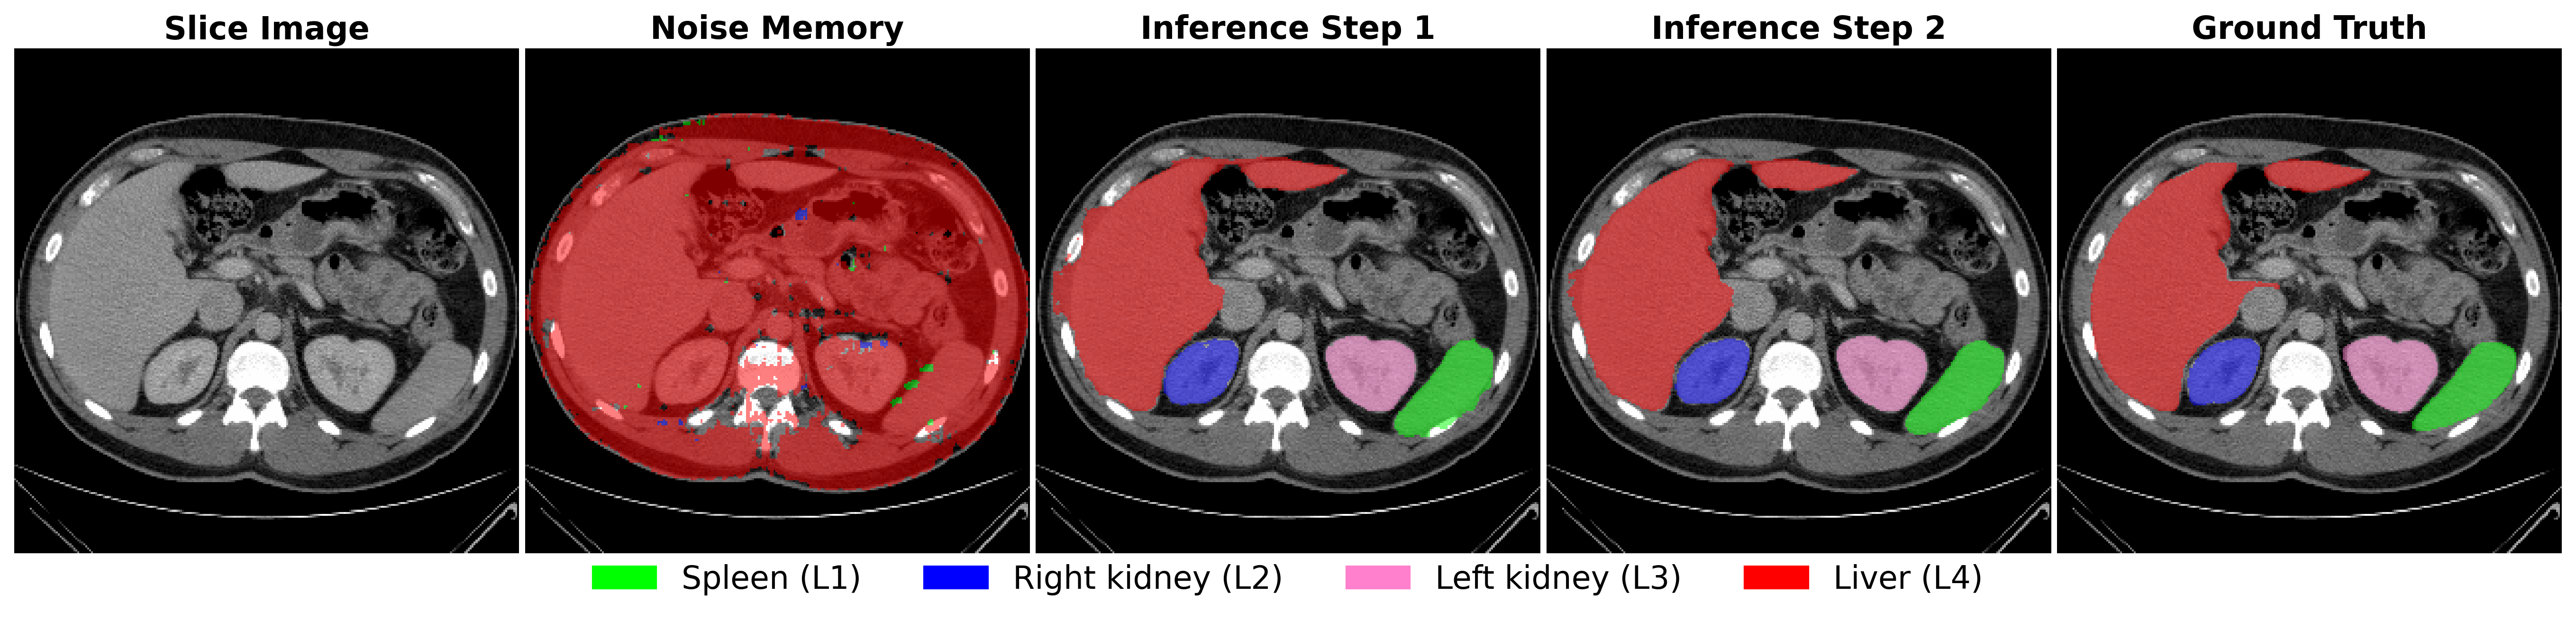
\includegraphics[width=0.88\columnwidth]{inference_steps_patient_36_slice_32.png}\\[2pt]
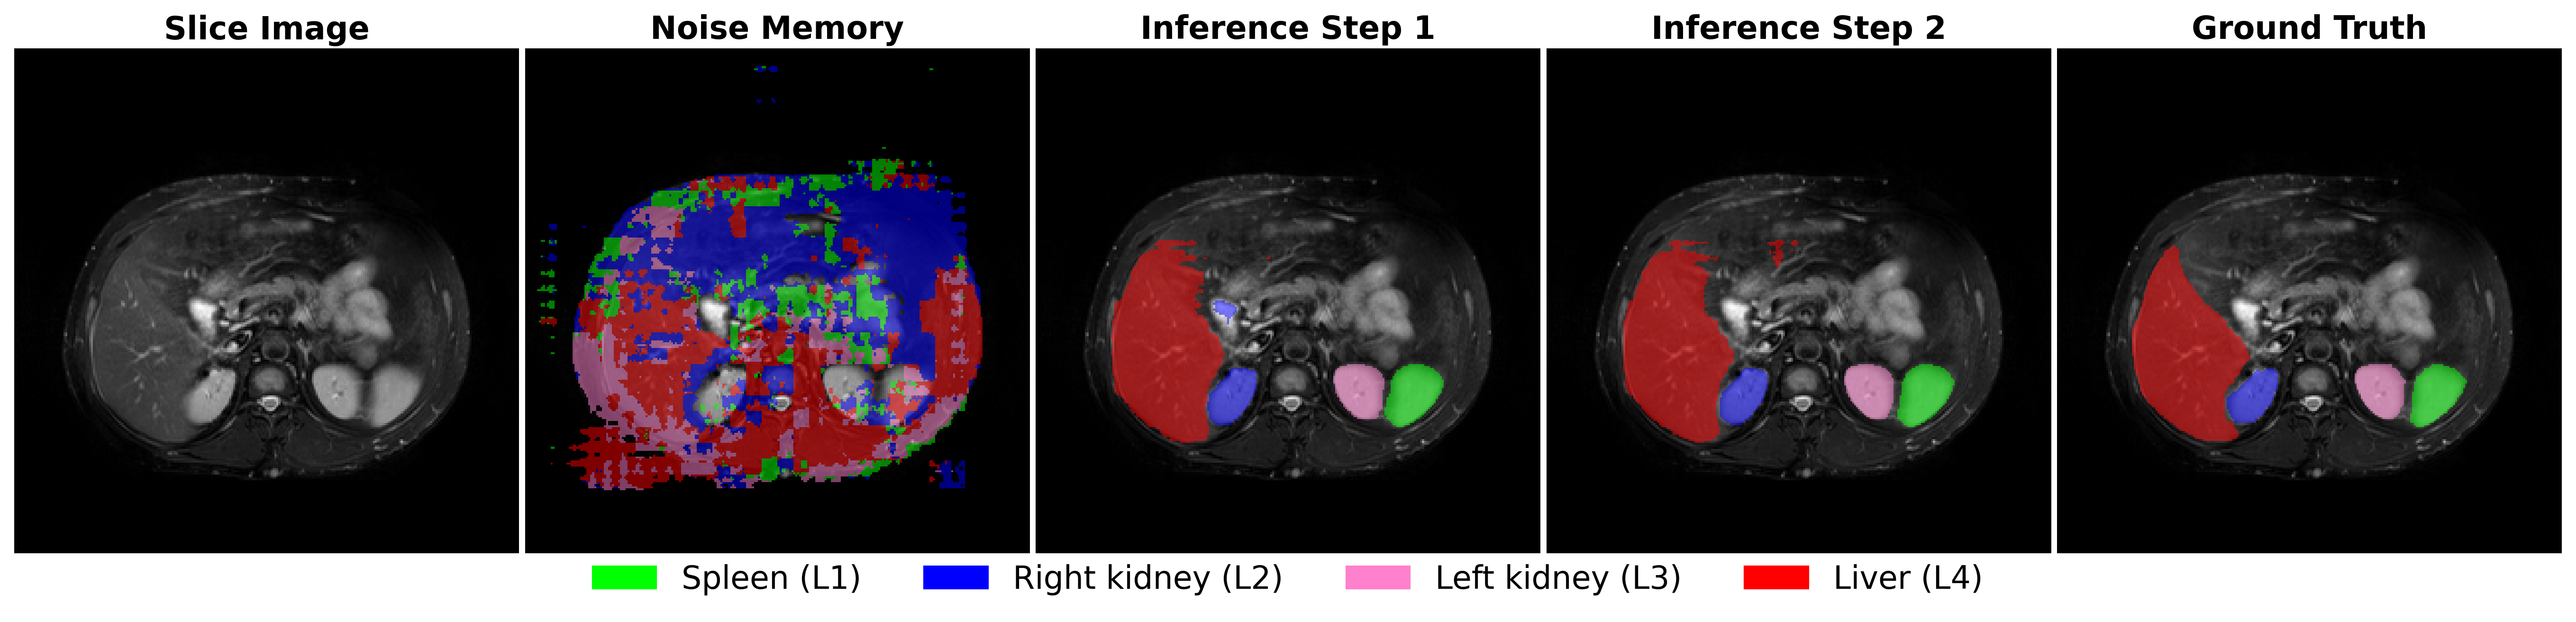
\includegraphics[width=0.88\columnwidth]{inference_steps_patient_IMG-0007-2_slice_10.png}
\end{center}
{\small\textit{Progressive diffusion refinement.} Top: CT (BTCV). Bottom: MRI (CHAOS). Accurate segmentations emerge in only 2 diffusion steps.}

% t-SNE AFTER inference (per plan)
\begin{center}
\begin{minipage}[t]{0.46\columnwidth}\centering
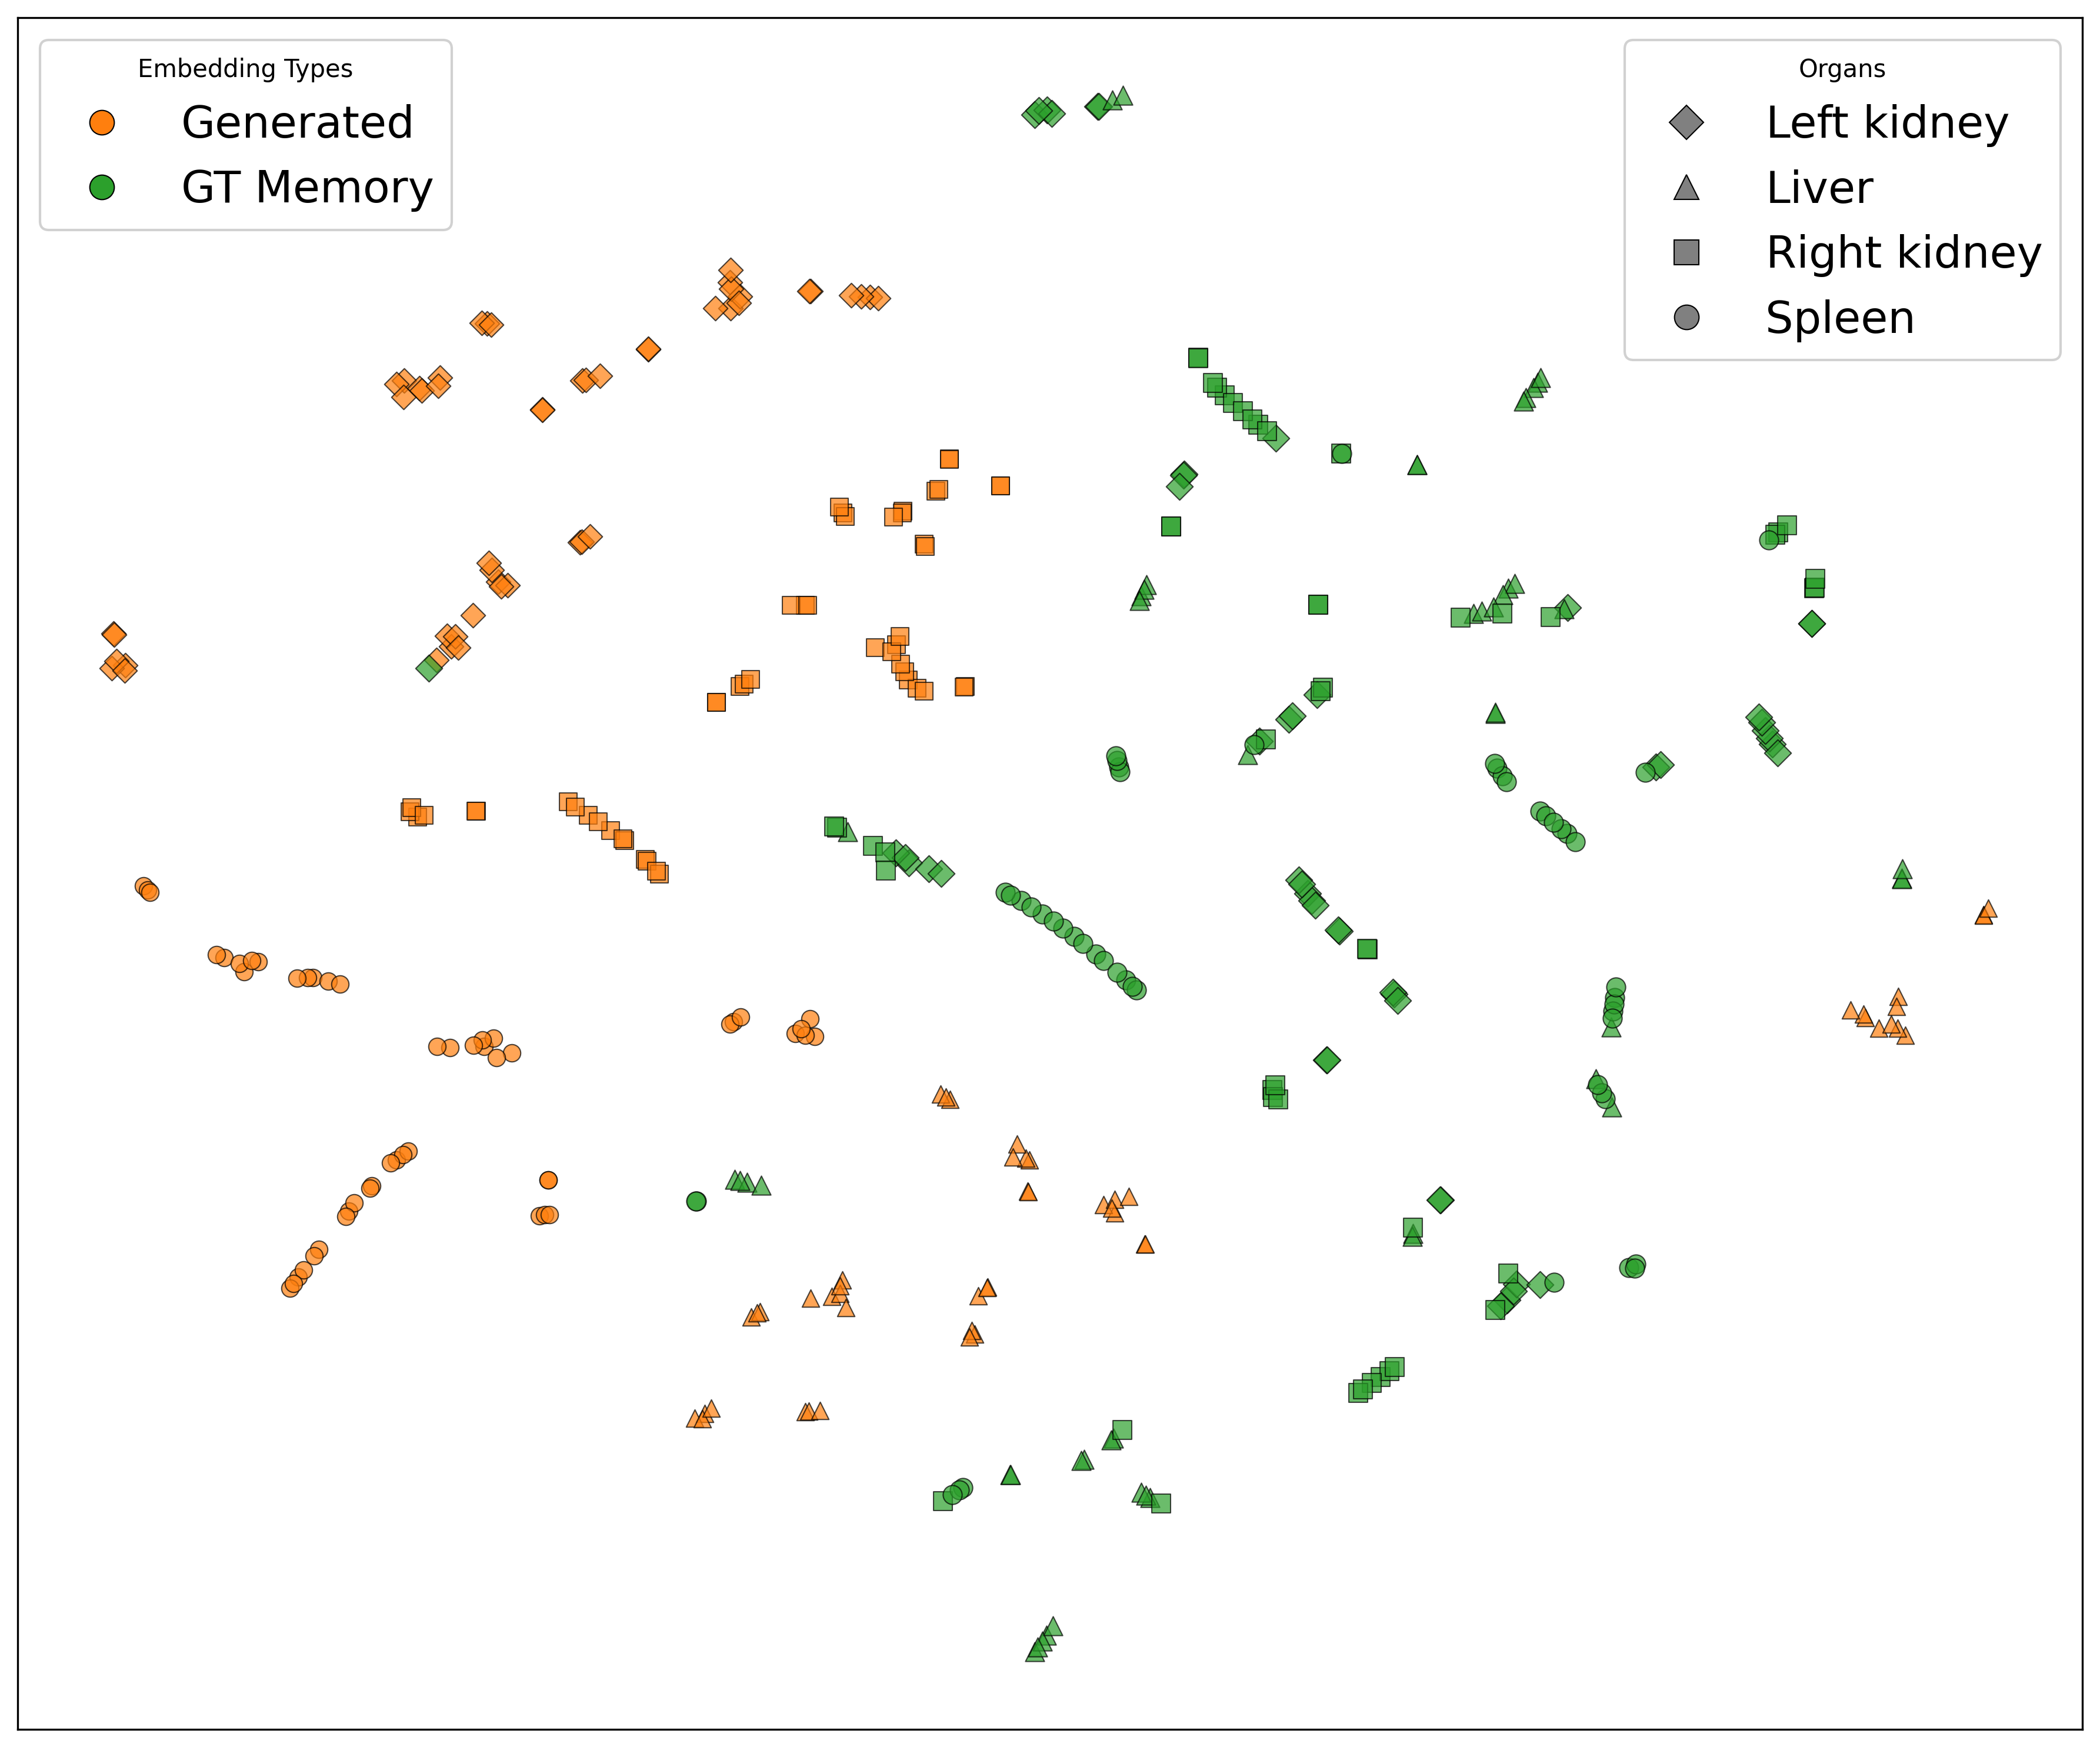
\includegraphics[width=\linewidth]{tsne_combined_all_organs_perp3_epoch1.png}\\[2pt]
{\small (A) Epoch 1}
\end{minipage}\hfill
\begin{minipage}[t]{0.46\columnwidth}\centering
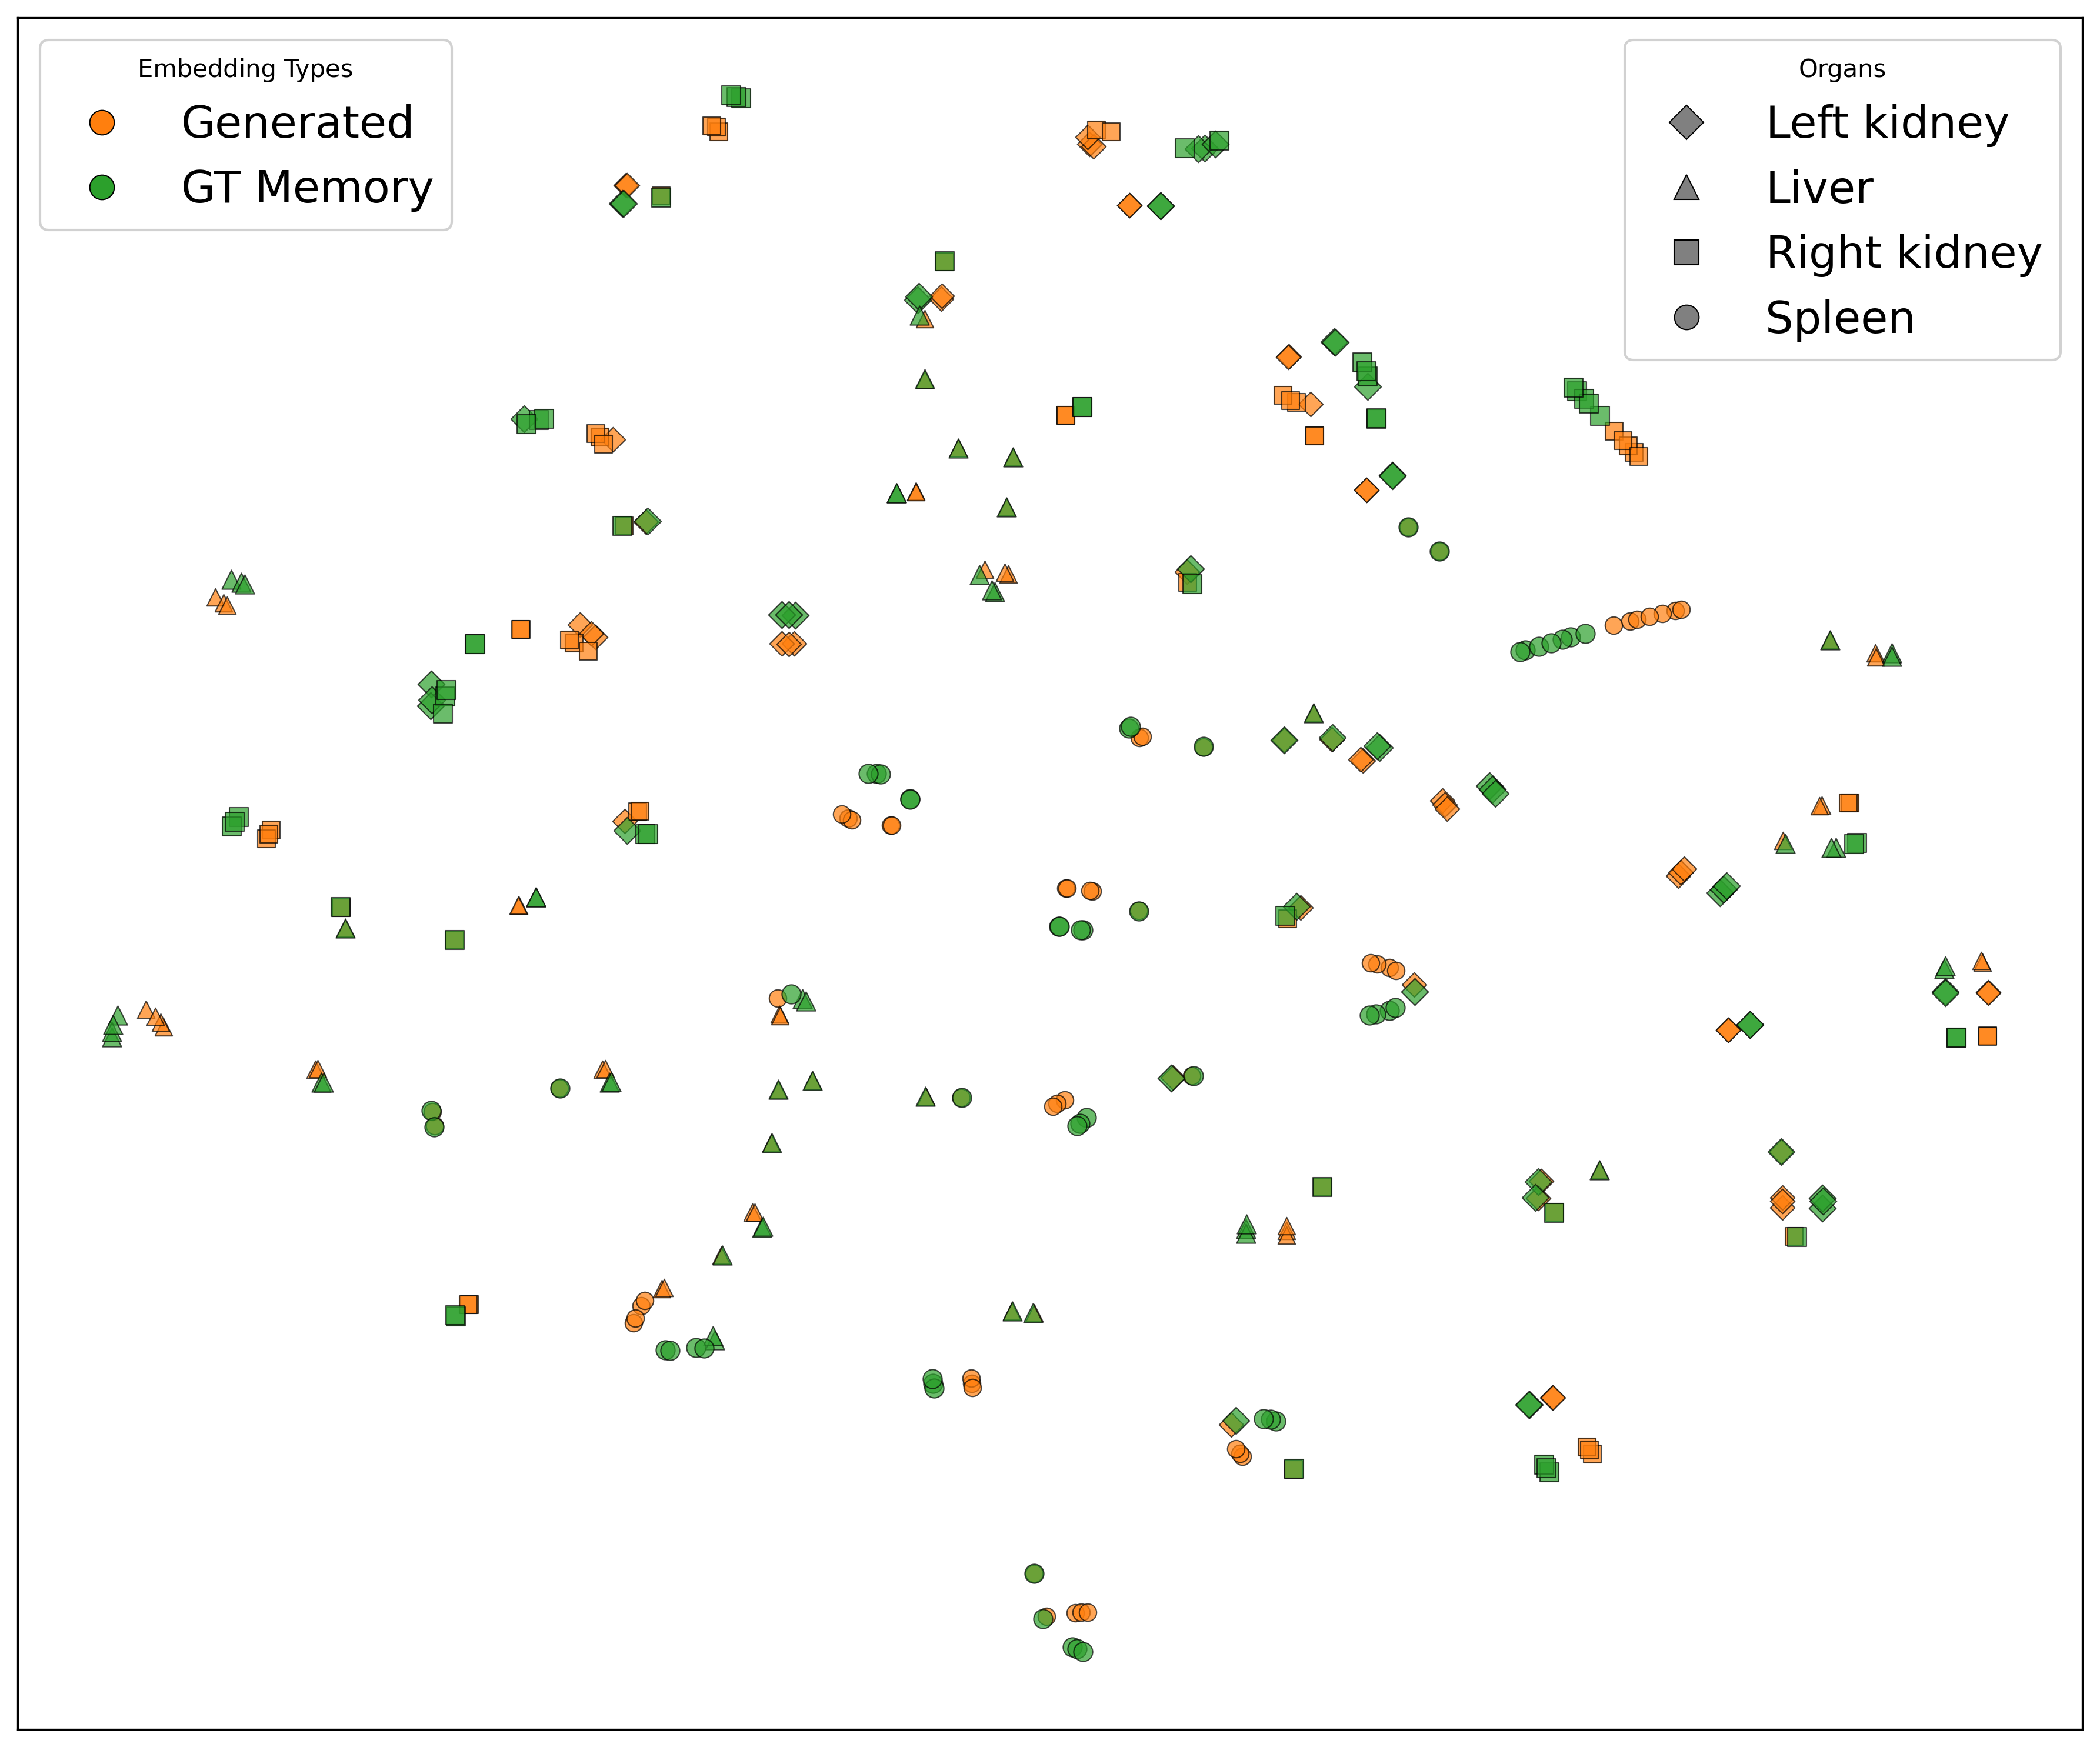
\includegraphics[width=\linewidth]{tsne_combined_all_organs_perp3_epoch75.png}\\[2pt]
{\small (B) Epoch 75}
\end{minipage}
\end{center}
{\small\textit{t-SNE of generated vs.\ ground-truth SAM2 memory embeddings.} (A) Early training: diffuse, misaligned. (B) End of training: compact, aligned clusters.}

\vspace{0.15cm}
\sectionbar{Discussion and Conclusion}

DiffuSAM demonstrates that a compact diffusion prior over frozen foundation model features enables competitive prompt-free segmentation with minimal training resources.
Current limitations include evaluation restricted to four abdominal organs across two datasets.
Future work will extend to broader anatomical structures and integrate additional domain adaptation strategies to support clinical deployment.

\vspace{0.15cm}
{\footnotesize
\colorbox{LightGray}{\parbox{\dimexpr\columnwidth-2\fboxsep}{%
\vspace{3pt}
\textbf{Keywords:}\enspace
Medical image segmentation,\enspace diffusion models,\enspace SAM2,\enspace prompt-free segmentation,\enspace source-free domain adaptation
\vspace{3pt}
}}
}
\sectionbar{References}

\vspace{0.12cm}
{\small
\begin{minipage}[t]{0.48\columnwidth}
\begin{enumerate}[leftmargin=1.15em, itemsep=1pt, topsep=1pt]
\item Kirillov A et al. \textit{arXiv} 2023;2304.02643.
\item Ravi N et al. \textit{arXiv} 2024;2408.00714.
\item Ma J et al. \textit{Nat Commun} 2024;15:654.
\item Ronneberger O et al. \textit{MICCAI} 2015:234--241.
\item Hatamizadeh A et al. \textit{WACV} 2022:574--584.
\end{enumerate}
\end{minipage}\hfill
\begin{minipage}[t]{0.48\columnwidth}
\begin{enumerate}[leftmargin=1.15em, itemsep=1pt, topsep=1pt, start=6]
\item He X et al. \textit{arXiv} 2025;2501.09138.
\item Huai Z et al. \textit{IEEE TMI} 2025.
\item Chen C et al. \textit{MICCAI} 2021:225--235.
\item Landman B et al. \textit{MICCAI Workshop} 2015.
\item Kavur AE et al. \textit{Med Image Anal} 2021;69:101950.
\end{enumerate}
\end{minipage}
}

\begin{center}
\includegraphics[width=0.22\columnwidth]{qrcode/qrcode_arxiv_diffusam.png}
\end{center}

\end{multicols}

\end{document}
